\section{Evaluación y resultados}
Se concluyó que el desarrollo de un sistema backend requiere de una arquitectura sólida (MVC) sustentada en un paradigma adecuado (POO), lo que garantiza la organización del software y su seguridad. Asimismo, la importancia de emplear una metodología debidamente estructurada (Scrum) permite adaptarse a los cambios y mejorar la comunicación.
Estos hallazgos no solo orientaron la decisión técnica hacia Spring Boot para el entorno empresarial, sino que también aportaron criterios prácticos para optimizar la colaboración del equipo y la calidad del producto desarrollado.

\subsection{Resultados en la arquitectura y el desarrollo del sistema Backend}
Se obtuvo un backend basado en la arquitectura Modelo-Vista-Controlador (MVC), implementado con Servicios RESTful que permiten:
Separación de Responsabilidades: El Controlador gestiona las peticiones HTTP y el Modelo maneja la lógica de negocio y la conexión a PostgreSQL.
Reutilización y Escalabilidad: La adopción de la Programación Orientada a Objetos (POO) con Spring Boot aportó principios como la reutilización y el encapsulamiento, garantizando un desarrollo más estructurado y con mayor facilidad para la mantenibilidad y evolución futura del sistema.
Seguridad Mejorada: La madurez de Spring Boot facilita la implementación de características de seguridad críticas, abordando vulnerabilidades comunes en aplicaciones web.

\begin{figure}[htbp]
    \centering
    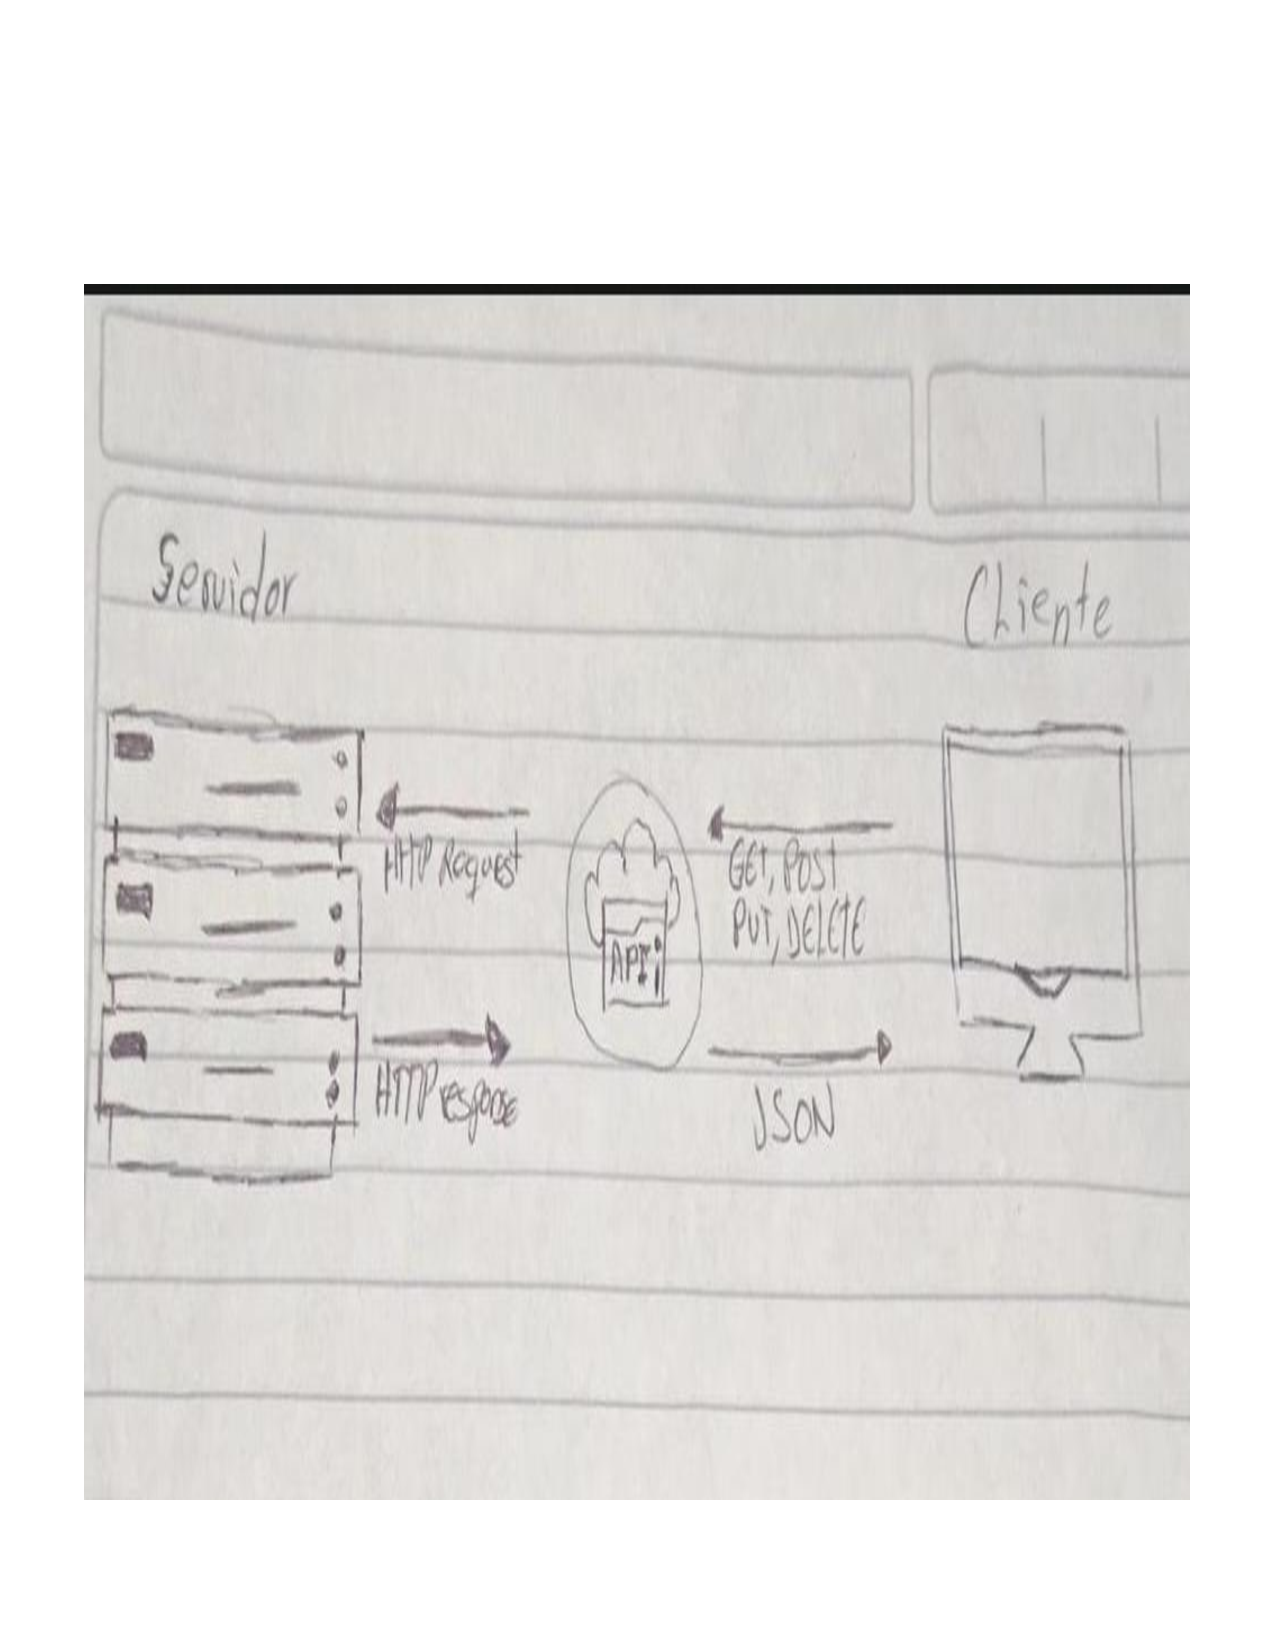
\includegraphics[width=0.48\textwidth]{graphics/SERVICIOS.pdf}
    \caption{Arquitectura de Servicios RESTful}
    \label{fig:servicios}
\end{figure}

En la Figura \ref{fig:servicios} se ilustra la arquitectura de comunicación de los servicios. Esta muestra cómo el API RESTful funciona como la capa central que media la transferencia de datos entre los servidores backend (donde reside la lógica) y la aplicación cliente. Este enfoque de servicios permitió la total desconexión del backend del frontend, facilitando la escalabilidad del sistema \cite{hernandez2015guia}.

\subsection{Resultados en la aplicación de la metodología ágil (Scrum)}
La implementación de la metodología ágil Scrum generó beneficios en la organización y el seguimiento del trabajo backend:
•	Planificación y Control: La organización en sprints y el uso de un tablero Kanban (e.g., Trello) permitieron la visualización clara de las tareas (diseño del API, implementación del Controlador, lógica del Modelo, pruebas).
•	Comunicación: Las reuniones de seguimiento fomentaron la comunicación constante y la responsabilidad compartida, esenciales para la resolución de bugs y la adaptación a cambios de requisitos.

\begin{figure}[htbp]
    \centering
    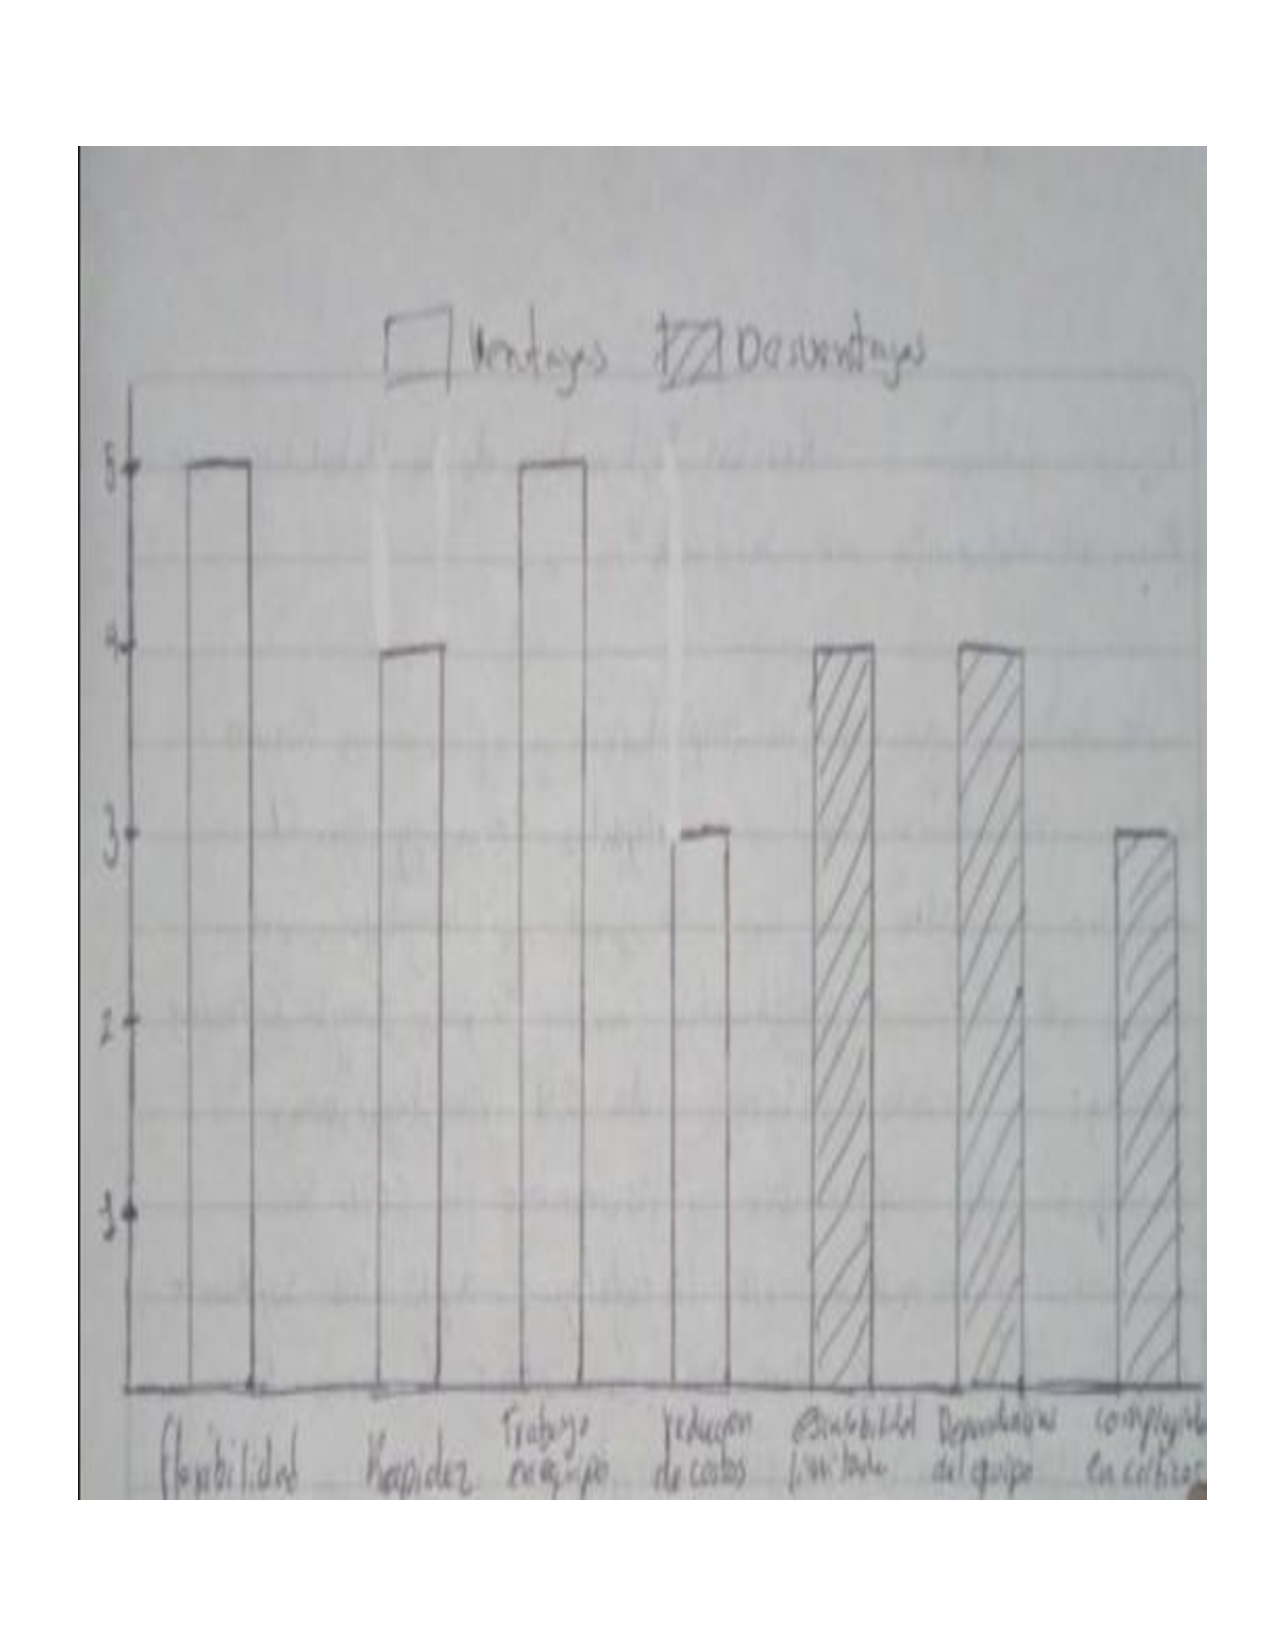
\includegraphics[width=0.48\textwidth]{graphics/DiagramaScrum.pdf}
    \caption{Diagrama de los beneficios de Scrum}
    \label{fig:scrum}
\end{figure}

En la Figura \ref{fig:scrum} se observa el diagrama de los beneficios de Scrum, que ilustra cómo esta metodología ágil mejora la planificación, control y comunicación en el desarrollo de proyectos backend \cite{brito_consideraciones}.
